\section{Автоморфизмы графа. Планарные графы. Поток на графе}
\subsection{Автоморфизм графа}
\begin{definition}
    \textbf{Граф} - это множество точек $V$ и множество ориентированных
     рёбер $\overrightarrow{E}$,
    на которых заданы отображения $S:\overrightarrow{E} \rightarrow V$ и $t:\overrightarrow{E} \rightarrow V$ такие,
    что $t(e)=v \Rightarrow \phi(t(e)) = \phi(v)$.
\end{definition}
\begin{explanation*}
    Вот, что такое отображения выше:
    \begin{itemize}
        \item $S:\overrightarrow{E} \rightarrow V$ - функция, возвращающая
        начало ребра
        \item$t:\overrightarrow{E} \rightarrow V$ - функция, возвращающая конец ребра
        \item Последние условие на отображения говорит нам о сохранении структуры графа
    \end{itemize}
\end{explanation*}

\begin{definition}
    \textbf{Изоморфизм графов} - это биективное отображение графа $G$ на граф $H$ с сохранением
    структуры.
\end{definition}
\begin{explanation*}
    Пусть $G, H$ - графы, тогда биективные отображения
        $$\phi : V_{G} \rightarrow V_{H}$$
        $$\psi : \overrightarrow{E}_{G} \rightarrow \overrightarrow{E}_{H}$$
задающие биекции, с сохранением структуры, задают изоморфизм.
\end{explanation*}
\textbf{Пример:} даны графы $G, H$ соответственно

\begin{tikzpicture}
    \begin{scope}[every node/.style={circle,thick,draw}]
        \node[shape=circle,draw=black] (A) at (0,1.5) {$a$};
        \node[shape=circle,draw=black] (B) at (-1.5,0) {$b$};
        \node[shape=circle,draw=black] (C) at (-1.25,-2) {$c$};
        \node[shape=circle,draw=black] (D) at (1.25,-2) {$d$};
        \node[shape=circle,draw=black] (E) at (1.5,0) {$e$};
    \end{scope}
    
    \begin{scope}[every node/.style={circle,thick,draw}]
    \path (A) edge (B);
    \path (A) edge (E);
    \path (B) edge (C);
    \path (E) edge (D);
    \path (D) edge (C);
    \end{scope}

    \begin{scope}[every node/.style={circle,thick,draw}]
        \node[shape=circle,draw=black] (A) at (6,1.5) {$\alpha$};
        \node[shape=circle,draw=black] (B) at (6-1.5,0) {$\varepsilon$};
        \node[shape=circle,draw=black] (C) at (6-1.25,-2) {$\delta$};
        \node[shape=circle,draw=black] (D) at (6+1.25,-2) {$\gamma$};
        \node[shape=circle,draw=black] (E) at (6+1.5,0) {$\beta$};
    \end{scope}
    \begin{scope}[every node/.style={circle,thick,draw}]
        \path (A) edge (D);
        \path (A) edge (C);
        \path (E) edge (B);
        \path (E) edge (C);
        \path (B) edge (D);
    \end{scope}

    \node[text width=6cm, anchor=west, right] at (7.5,0)
    {
        \begin{multline*}
            \phi : V_{G} \rightarrow V_{H}\text{ - биективное отображение, тогда:}\\
            \phi(a) = \alpha,\\
            \phi(b) = \gamma, \\
            \phi(c) = \varepsilon, \\
            \phi(d) = \beta, \\
            \phi(e) = \delta\\
        \end{multline*}
    };
\end{tikzpicture}
\\
\begin{definition}
    \textbf{Автоморфизм} - изоморфизм графа с собой.
\end{definition}

\textbf{Пример:}

\begin{tikzpicture}
    \begin{scope}
        \node[shape=circle,draw=black] (A) at (0,0) {$A$};
        \node[shape=circle,draw=black] (B) at (4,0) {$B$};
        \node[text width=6cm, anchor=north, right] at (0, -1){Это 
        очень простой граф};
        \node[text width=8cm, anchor=east, right] at (6, 0){
            Определим два отображения, задающих автоморфизм:\begin{enumerate}
                \item $\phi(a) = a$, $\phi(b) = b$\\ т.е. $\phi=Id$ ($Id$ - тождественное отображение) 
                \item $\psi(a) = b$, $\psi(b) = a$\\ $\psi$ - \textbf{автоморфизм}, но не тождественное
                отображение
            \end{enumerate}
        };
    \end{scope}
    \begin{scope}
        \path (A) edge (B);
    \end{scope}
    % \draw[red, thick][->] (1,1) arc (0:360:0.5);
    % \draw[black, ultra thick][<-] (1,1) arc (0:360:1);
    % \fill[yellow] (1,1) circle (2pt);
\end{tikzpicture}
\newpage
Теперь займёмся подсчётом \textbf{автоморфизмов}(симметрий, но не в школьном понимании) в более сложных графах:
\begin{enumerate}
    \item 
    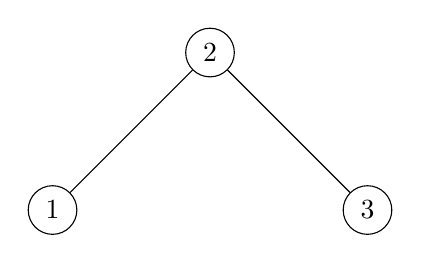
\begin{tikzpicture}
        \begin{scope}
            \node[shape=circle, draw=black] (1) at (2,0) {2};
            \node[shape=circle, draw=black] (2) at (0,-2) {1};
            \node[shape=circle, draw=black] (3) at (4,-2) {3};
            %\node[text width=12cm, anchor=east, right] at (6, 0){};
        \end{scope}
        \begin{scope}
            \path (1) edge (2);
            \path (1) edge (3);
        \end{scope}
    \end{tikzpicture}
    \begin{claim*}
        Вершина №2 может отображаться только в себя, т.к. у неё единственной в множестве вершин этого графа
        2 валентности. Вершины №1 и №3 могут отображаться как в себя, так и в друг друга, поэтому имеем два автоморфизма:
        тождественный и задающийся подстановкой 
        $\begin{pmatrix}
            1&2&3\\
            3&2&1
        \end{pmatrix}$.

        Получим, что группа автоморфизмов графа имеет мощность 2, и состоит соответственно из тождественного
        отображения и указанной выше подстановки:
        $$
        AutG = \{Id, 
        \begin{pmatrix}
            1&2&3\\
            3&2&1
        \end{pmatrix}
        \}
        $$
    \end{claim*}
    \begin{explanation*}
        Можно подумать и по-другому. Автоморфизм отображает не только вершины, но и рёбра, поэтому давайте 
        размыслим в категориях рёбер: сколькими способами можно переставить рёбра в заданном графе так, 
        чтобы не изменить его структуру, т.е. так, чтобы у каждого ребра сохранилось количество инцидентных 
        ему рёбер и его направление? Имеем, что рёбра могут быть отражены зеркально относительно вершины №2
        или же остаться на месте, т.е. имеем всего 2 варианта. Это и есть ответ.
    \end{explanation*}
    \item 
    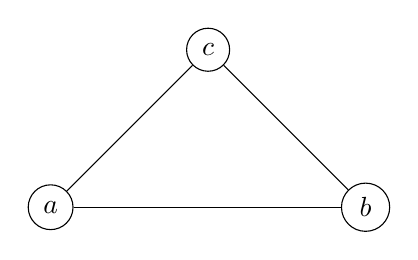
\begin{tikzpicture}
        \begin{scope}
            \node[shape=circle, draw=black] (1) at (2,0) {$c$};
            \node[shape=circle, draw=black] (2) at (0,-2) {$a$};
            \node[shape=circle, draw=black] (3) at (4,-2) {$b$};
            %\node[text width=12cm, anchor=east, right] at (6, 0){};
        \end{scope}
        \begin{scope}
            \path (1) edge (2);
            \path (1) edge (3);
            \path (2) edge (3);
        \end{scope}
    \end{tikzpicture}
    \begin{claim*}
        Каждая из вершин имеет по три валентности, следовательно, без нарушения структуры она может отобразиться в себя
        и в любую соседнюю вершину. Имеем $3!$ возможностей и $|AutG| = 6$.
    \end{claim*}
    \item 
    \begin{tikzpicture}
        \begin{scope}
            \node[shape=circle, draw=black] (1) at (2,-2) {2};
            \node[shape=circle, draw=black] (2) at (0,0) {1};
            \node[shape=circle, draw=black] (3) at (4,0) {3};
            \node[shape=circle, draw=black] (4) at (2,-4) {4};
            %\node[text width=12cm, anchor=east, right] at (6, 0){};
        \end{scope}
        \begin{scope}
            \path (1) edge (2);
            \path (1) edge (3);
            \path (1) edge (4);
        \end{scope}
    \end{tikzpicture}
    \begin{claim*}
        Вершина №2 единственная с тремя валентностями, поэтому отображаться с сохранением
        структуры она может только в себя. Остальные вершины могут без ограничений отображаться
        друг в друга, поэтому имеем ситуацию как с треугольником выше.
    \end{claim*}
    \begin{notice}
        Петля на самом деле имеет два автоморфизма:
        \begin{center}
            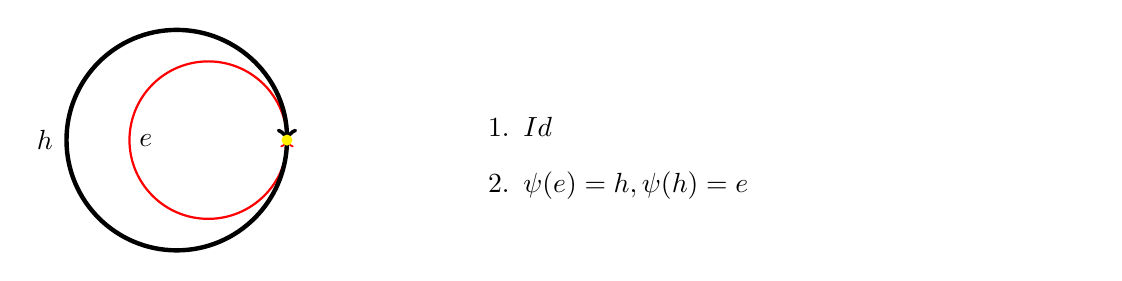
\begin{tikzpicture}
                \begin{scope}
                    \draw[red, thick][->] (1,1) arc (0:360:1);
                    \draw[black, ultra thick][<-] (1,1) arc (0:360:1.4);
                    \fill[yellow] (1,1) circle (2pt);
                \end{scope}
                \begin{scope}
                    \node[text width=2cm, anchor=west, right] at (-2.3,1){$h$};
                    \node[text width=2cm, anchor=west, right] at (-1,1){$e$};
                    \node[text width=8cm, anchor=west, right] at (3,1){
                    \begin{enumerate}
                        \item $Id$
                        \item $\psi(e) = h, \psi(h) = e$
                    \end{enumerate}
                    };
                \end{scope}
            \end{tikzpicture}
        \end{center}
    \end{notice}
    \item
    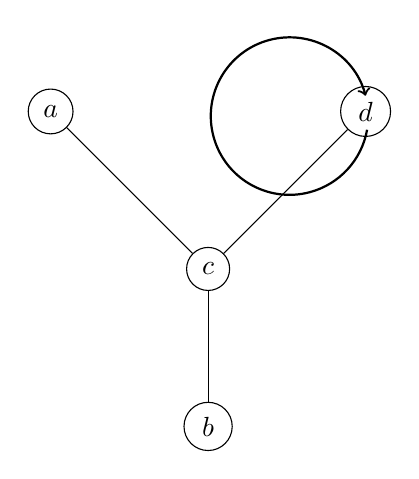
\begin{tikzpicture}
         \begin{scope}
            \draw[black, thick][<-] (4,0.2) arc (15:350:1);
        \end{scope}
        \begin{scope}
            \node[shape=circle, draw=black] (1) at (2,-2) {$c$};
            \node[shape=circle, draw=black] (2) at (0,0) {$a$};
            \node[shape=circle, draw=black] (3) at (4,0) {$d$};
            \node[shape=circle, draw=black] (4) at (2,-4) {$b$};
            %\node[text width=12cm, anchor=east, right] at (6, 0){};
        \end{scope}
        \begin{scope}
            \path (1) edge (2);
            \path (1) edge (3);
            \path (1) edge (4);
        \end{scope}
    \end{tikzpicture}
    \begin{claim*}
        Петлю можно повернуть двумя способами, вершина $c$ может отобразиться только в себя - см. предыдущий пункт - остаётся 
        перестановка вершин $a$ и $b$ - их можно расставить двумя способами:
        не перемещая или отобразив друг в друга. Итого $2*2=4$.
    \end{claim*}
    \item 
    \begin{tikzpicture}
        \begin{scope}
            \node[shape=circle, draw=black] (1) at (0,0) {1};
            \node[shape=circle, draw=black] (2) at (2,-2) {2};
            \node[shape=circle, draw=black] (3) at (6,-2) {3};
            \node[shape=circle, draw=black] (4) at (8,0) {4};
            \node[shape=circle, draw=black] (5) at (8,-4) {5};
            \node[shape=circle, draw=black] (6) at (0,-4) {6};
        \end{scope}
        \begin{scope}
            \path (1) edge (2);
            \path (2) edge (3);
            \path (3) edge (4);
            \path (3) edge (5);
            \path (6) edge (2);
        \end{scope}
    \end{tikzpicture}
    \begin{claim*}
        Вершины №2 и №6 можно расставить двумя способами. Аналогично с вершинами №4 и №5.\\
        Теперь про вершины №2 и №3: здесь важно, чтобы отображение вершины №2 было инцидентно ребрам, на которые отобразились вершины №1 и №6. Аналогичное условие накладывается на вершину №3. Поэтому для них есть только 2 возможности: либо они отображаются в себя, либо мы отражаем граф относительно центра ребра, соединяющего вершины №2 и №3. \textbf{Итого:} $2*2*2=8$ отображений.
    \end{claim*}
    \item
    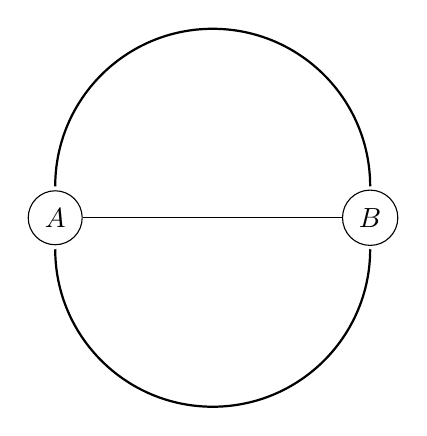
\begin{tikzpicture}
    \begin{scope}
        \node[shape=circle,draw=black] (A) at (0,0) {$A$};
        \node[shape=circle,draw=black] (B) at (4,0) {$B$};
    \end{scope}
    \begin{scope}
        \path (A) edge (B);
        \draw[black, thick] (4,0.4) arc (0:180:2);
        \draw[black, thick] (0,-0.4) arc (180:360:2);
    \end{scope}
\end{tikzpicture}
\begin{claim*}
    Все три ребра здесь идентичны, поэтому берём сразу $3!$ способа их расставить. Но их можно ещё и перевернуть, поэтому добавляется ещё 2 варианта. \textbf{Итого:} $3!*2=12$ вариантов.
\end{claim*}
\end{enumerate}